\documentclass[a4paper,11pt]{article}

\usepackage{latexsym}
\usepackage{graphicx}
\usepackage{float}
\usepackage[margin=2cm]{geometry}
\usepackage{lscape}
\usepackage{underscore}
\usepackage{amsmath}
\usepackage{blindtext}
\usepackage{listings}
\usepackage{xcolor}
\usepackage{mathtools}
\usepackage{comment}

\usepackage[all]{nowidow}

\usepackage[LY1]{fontenc}
\usepackage[utf8x]{inputenc}
\usepackage{polski}
\usepackage[lf,enc=t1]{berenis}

\DeclareTextCompositeCommand{\k}{LY1}{a}
  {\oalign{a\crcr\noalign{\kern-.27ex}\hidewidth\char7}}


\begin{document}

\tableofcontents
\newpage

\section{Wspomagane wyszukiwanie drużyn - wstęp teoretyczny}

\subsection{Problem optymalizacji wielokryterialnej}

Problem optymalizacji wielokryternialnej jest rozszerzeniem problemu optymalizacji jednokryternialnej, gdzie poszukiwana jest decyzja optymalna, ze zbioru możliwych decyzji na podstawie jednego kryterium. Problem ten sprowadza się do poszukiwania maksimum (bądź minimum) funkcji  oceny danego kryterium. Jeżeli kryterium jest ilościowe, np. maksymalna prędkość samochodu, to podejmując decyzję o zakupie jedynie ze względu na to kryterium naturalnie wybierzemy samochód, który osiąga największą prędkość.

Często jednak podjęcie decyzji może być uwarunkowane większą ilością czynników, na przykład, w przypadku samochodu może to być jego cena, koszt utrzymania, czy czynniki nie ilościowe takie jak jego kolor (w zależności od preferencji kupca). Podejmując decyzję należy rozpatrzyć wiele kryteriów oraz relacje między nimi. Decyzja, która jest optymalna ze względu na jedno z kryteriów, nie musi być optymalną ze względu na pozostałe - z reguły tak nie jest. 

W literaturze można znaleźć wiele sposóbów na rozwiązywanie tego typu problemu. W dalszej częsci pracy zostanie wybrany sposób, który najbardziej pasuje do domeny problemu.


\subsubsection{Tradycyjny sposób rozwiązywania problemu}

Tradycyjne algorytmy składają się z dwóch etapów. W pierwszej kolejności następuje normalizacja wartości kryteriów, a następnie agregacja, której wynikiem jest decyzja optymalna. 

\begin{figure}[H]
\centering
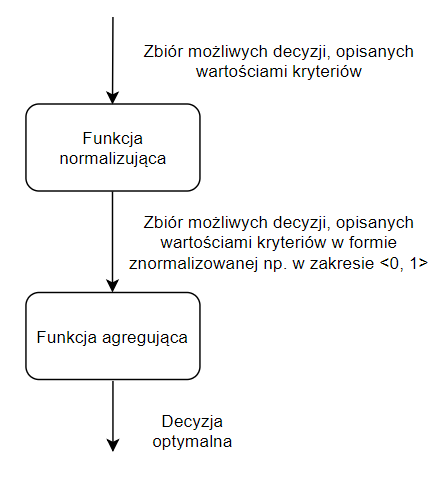
\includegraphics[width=9cm]{tradycyjne-algorytmy-opt.PNG}
\caption{Ogólny schemat metody rozwiązywania problemu optymalizacji wielokryterialnej}
\end{figure}

\subsubsection{Normalizacja - metody liniowe}

Tradycyjnymi metodami normalizacji kryteriów są metody normalizacji liniowej. W wyniku przekształceń wartości kryteriów zostają znormalizowane do przedziału wartości <0, 1>.
\begin{table}[H]
\centering
\label{tbl:excel-table}
\caption{Liniowe metody normalizacji kryteriów \cite{pa}}
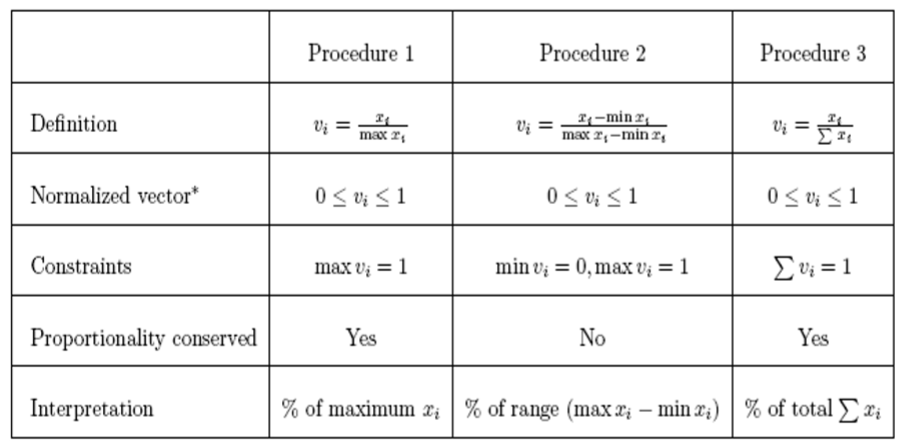
\includegraphics[width=15cm]{linear-normalization.PNG}
\end{table}


\subsubsection{Agregacja - Metoda ważonych kryteriów}

Metoda ważonych kryteriów polega na opisaniu funkcji oceny decyzji jako sumy ważonej ocen poszczególnych kryteriów. Konieczne jest przyporządkowanie wagi dla każdego z kryteriów. Ocena poszczególnych decyzji obliczana jest według wzoru: 

<< Wstawić wzór>>

\subsection{Lokalizacja problemu w projektowanym systemie}

Jednym z podstawowych zadań systemu jest wspomaganie wyboru przeciwników. System powinien zaproponować kapitanowi drużyny listę sugerowanych rywali będącą jak najbardziej dopasowaną do jego preferencji. Można zdefiniować wiele kryteriów, które wpływają na jakość dopasowania. Moga to być m.in średni wiek zawodników, łączny staż gry, odległość punktów macierzystych drużyn, pokrycie preferowanych godzin gry, poziom fair play drużyny przeciwnej, ocena poprzednich rozgrywek z daną drużyną, poziom rankingowy w systemie. 

\subsubsection{Wymagania czasowe dla algorytmu}

System musi być w stanie dokonać oceny przeciwników w rozsądnym czasie. Rozsądnym limitem czasowym jaki kapitan może oczekiwać na wynik działania systemu jest 5 sekund. Wyszukiwanie przeciwników będzie odbywać się dla konkretnej dyscypliny sportu oraz regionu. Biorąc pod uwagę skalę systemu, można założyć, że w danym regionie nie powinno być więcej aniżeli 5000 drużyn. W przypadku większych regionów powinny one zostać podzielone na mniejsze podregiony. Z tych ustaleń wynika, że zaproponowany oraz zaimplementowany algorytm powinien być w stanie przetworzyć 5000 drużyn w czasie nie większym niż 5 sekund. Zaimplementowany algorytm zostanie przetestowany pod kątem tych ograniczeń.

\subsubsection{Propozycja algorytmu - ogólny schemat}

Proponując algorytm należy mieć na uwadzę domenę problemu oraz charakter danych, na jakich będzie on operował. W związku z tym do tradycyjnego schematu oceny rozwiązań zostanie wprowadzona modyfikacja.

 Normalizacja poszczególnych kryteriów będzie przebiegać przy użyciu różnych funkcji, dopasowanych do charakteru danych. Przykładem uzasadniającym konieczność zastosowania takiej modyfikacji może być porównanie dwóch kryteriów: odległości drużyn oraz średniego wieku zawodników. O ile kryterium odległości może być normalizowane w pełni liniowo, o tyle dla różnicy wieku taka metoda normalizacji jest błędna. Różnica wieku między dwoma zawodnikami, którzy mają 15 oraz 20 lat jest znacznie bardziej istotna aniżeli różnica między zawodnikami w wieku 30 oraz 35 lat - nie można tutaj zastosować operatora liniowego. Dodatkowo w domenie problemu można wyróżnić kryteria nieliczbowe - cechy drużyny, które mogą mieć duży wpływ na jakość dopasowania, np. zadeklarowana chęć ponownej gry z daną drużyną.   

Jako funkcja agregujaca wybrana została tradycyjna metoda ważonych kryteriów ze względu na możliwość dynamicznego doboru wag poszczególnych kryteriów. Nietóre z tych wag będą dobierane przez kapitana zgodnie z preferencjami jego drużyny.

Na schemacie (Rysunek 2.) został przedstawiony ogólny schemat algorytmu. Symbole c1, c2, c3 oznaczają przykładowe kryteria.

\begin{figure}[H]
\centering
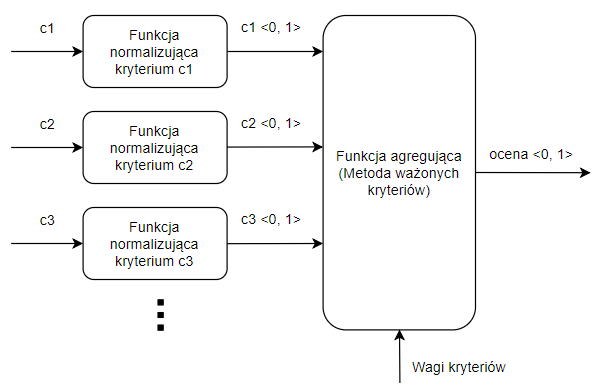
\includegraphics[width=15cm]{algorytm-2.PNG}
\caption{Uogólniony schemat algorytmu oceny decyzji}
\end{figure}




\begin{thebibliography}{99}
\bibitem{pa}dr hab. Mieczysław Połoński prof. SGGWl:
\emph{Analiza wielokryterialna – wstęp do zagadnienia}
\bibitem{pb}Lucia Vavríková,  Department of Mathematics, Faculty of Civil Engineering, Slovak University of Technology:
\emph{Multicriteria Decision Making and Rankings Based on Aggregation Operators}
\end{thebibliography}

\end{document}